\chapter{Dataset and Preprocessing}
\label{chap:data}

\section{The FLARE22 Dataset}

The FLARE22 (Fast and Low GPU-memory Abdominal oRgan sEgmentation 2022) dataset consists of
50 abdominal CT volumes with voxel-level annotations for 13 organs. Volumes are stored in
NIfTI format and vary in slice count, voxel spacing, and field of view. Table~\ref{tab:dataset}
summarises the dataset characteristics.

\begin{table}[h!]
\centering
\caption{FLARE22 dataset summary.}
\label{tab:dataset}
\begin{tabular}{ll}
\toprule
\textbf{Property} & \textbf{Value} \\
\midrule
Total annotated volumes          & 50 \\
Number of organ classes          & 13 \\
Total label classes (incl.\ background) & 14 \\
CT format                        & NIfTI (.nii.gz) \\
Approximate axial slice range    & 80--400 per volume \\
In-plane resolution              & $256 \times 256$ (after resize) \\
Typical voxel spacing (in-plane) & 0.72--0.82~mm \\
Typical slice thickness          & 2.5~mm \\
Training volumes                 & 42 \\
Validation volumes               & 8 \\
\bottomrule
\end{tabular}
\end{table}

\noindent
The 13 annotated organs are: liver (label~1), right kidney (2), spleen (3), pancreas (4),
aorta (5), inferior vena cava (6), right adrenal gland (7), left adrenal gland (8), gallbladder
(9), esophagus (10), stomach (11), duodenum (12), and left kidney (13).

\section{Class Imbalance}

Abdominal CT segmentation is severely imbalanced. The liver alone accounts for roughly
40--50\% of all foreground voxels, while each adrenal gland occupies less than 0.2\%.
Figure~\ref{fig:dataset_stats} illustrates the relative class frequencies in the FLARE22
training set. This imbalance directly informs the choice of a combined cross-entropy and
Dice loss (Chapter~\ref{chap:methodology}): the Dice component provides a natural normalisation
per class, preventing the liver from dominating gradient updates at the expense of smaller organs.

\begin{figure}[h!]
\centering
\begin{minipage}{0.85\textwidth}
  \centering
  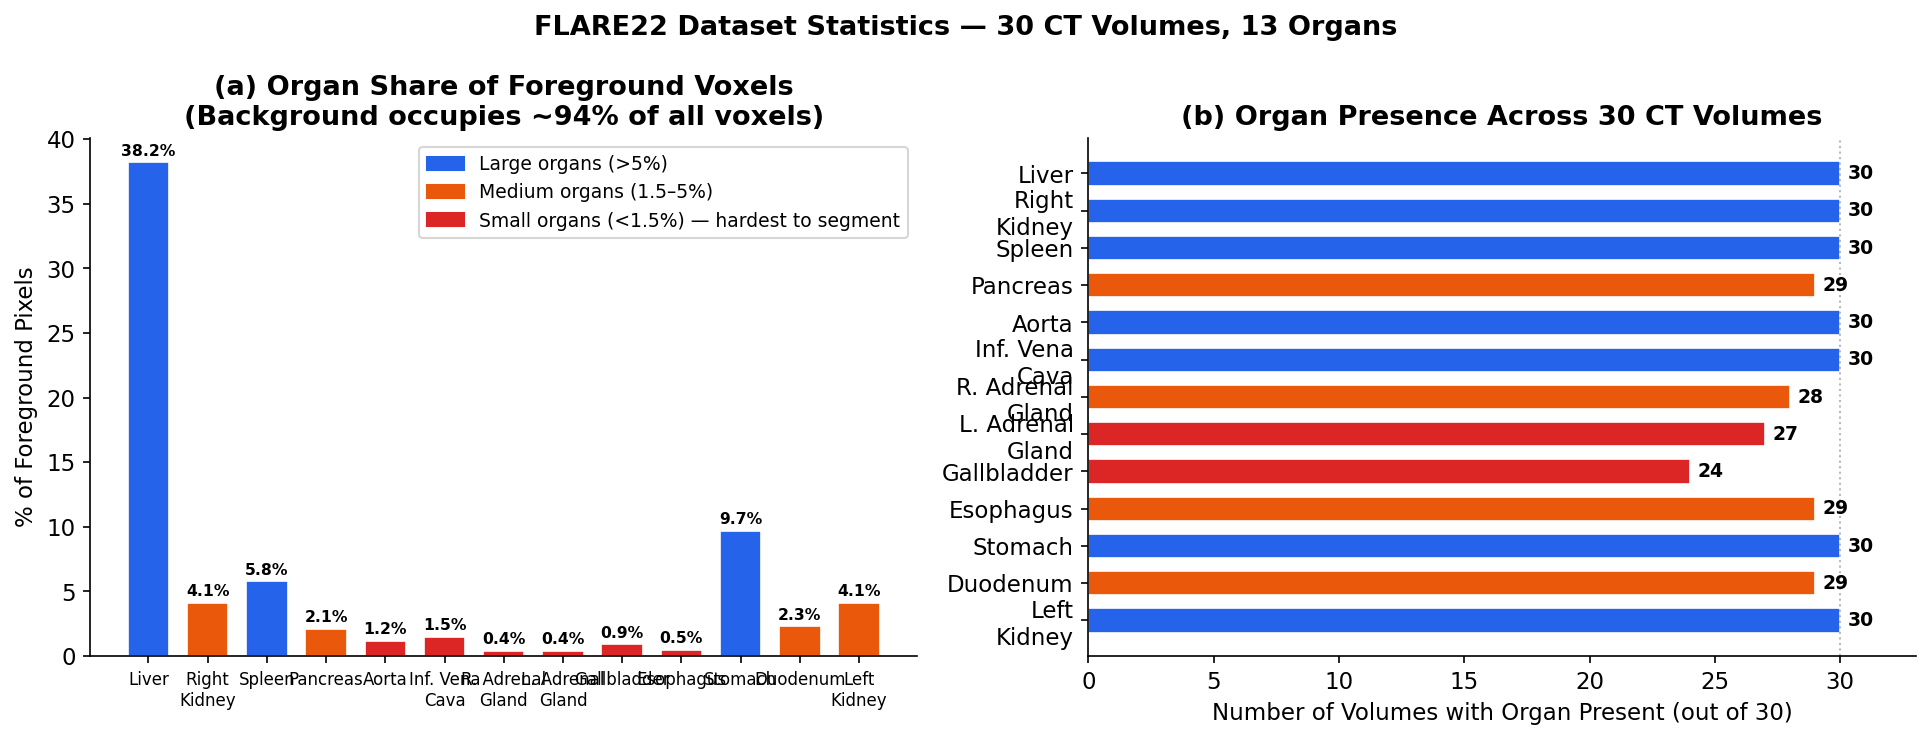
\includegraphics[width=\textwidth]{figures/fig_dataset_stats}
  \caption{Per-organ voxel frequency in the FLARE22 training set. The liver contributes the
  largest share of foreground voxels; adrenal glands, esophagus, and duodenum each represent
  less than 1\% of foreground.}
  \label{fig:dataset_stats}
\end{minipage}
\end{figure}

\FloatBarrier

\section{Train / Validation Split}

All 50 volumes are split at the volume level: 42 volumes for training and 8 for validation,
as summarised in Table~\ref{tab:split}. Volume-level splitting is essential --- a per-slice
split would allow slices from the same patient to appear in both sets, creating data leakage
that inflates validation metrics. The split was fixed before any training run to ensure
comparability across the ablation experiments (Runs~014--017).

\begin{table}[h!]
\centering
\caption{Volume-level train/val split.}
\label{tab:split}
\begin{tabular}{lcc}
\toprule
\textbf{Set} & \textbf{Volumes} & \textbf{Approximate Slices} \\
\midrule
Training   & 42 & 3{,}785 \\
Validation & 8  &   754   \\
Total      & 50 & 4{,}539 \\
\bottomrule
\end{tabular}
\end{table}

\section{Preprocessing Pipeline}

Each CT volume is preprocessed through the following steps before slices are extracted:

\begin{enumerate}
    \item \textbf{HU Windowing.}  Voxel intensities are clipped to the soft-tissue window
          $[-175, 250]$ Hounsfield Units, suppressing bone (HU $>$ 400) and air (HU $<$ $-1000$)
          that add noise without aiding organ discrimination.
    \item \textbf{Normalisation.}  Clipped intensities are linearly rescaled to $[0, 1]$.
    \item \textbf{Slice Extraction.}  Each axial slice is extracted as a 2D array together
          with its corresponding label mask.
    \item \textbf{Resize.}  Slices are bilinearly resized to $256 \times 256$ pixels; masks use
          nearest-neighbour interpolation to preserve integer labels.
    \item \textbf{Channel Expansion.}  Each 2D slice is replicated across 3 channels to match
          the expected input shape of the encoder.
\end{enumerate}

\section{Data Augmentation}

Augmentation is applied on-the-fly during training to reduce overfitting. The augmentation
strategy focuses on spatial transforms that preserve label integrity:

\begin{itemize}
    \item \textbf{Random horizontal flip} (probability 0.5)
    \item \textbf{Random vertical flip} (probability 0.5)
    \item \textbf{Random rotation} ($\pm 10^\circ$, nearest fill for masks)
    \item \textbf{Random brightness and contrast jitter} (factors drawn from $[0.8, 1.2]$)
\end{itemize}

No elastic deformations were applied in Run~017; the ablation study (Chapter~\ref{chap:ablation})
indicates that the chosen augmentation set is sufficient to avoid overfitting at 60 epochs
without risk of generating anatomically implausible training samples.
